\documentclass{article}
\usepackage{listings}
\usepackage{graphicx}
\usepackage[slovene]{babel}
\usepackage{color}
\usepackage{amsmath}
\usepackage{amssymb}
\usepackage{amsfonts}
\usepackage[usenames,dvipsnames]{xcolor}
\usepackage[hidelinks]{hyperref}
\usepackage{subcaption}
\usepackage{float}
\usepackage{rotating} 
\usepackage{hyperref}
\usepackage{caption}
\usepackage{siunitx}
\usepackage[margin=3cm]{geometry}
\usepackage[backend=biber,sorting=none]{biblatex}

\graphicspath{{./images/}}
\addbibresource{literature.bib}

\setlength{\parindent}{0pt}

\begin{document}

\title{Industrijska fizika \\[3mm] \large Transkodiranje NOAA APT signala}
\author{Luka Papež}
\date{25.\ julij 2025}

\begin{center}
    
\includegraphics[width=8cm]{logo-fmf.png}
\end{center}

{
    \let\newpage\relax
    \maketitle
}

\newpage
\section{Uvod}
V tem poročilu je predstavljen postopek enkodiranja in dekodiranja NOAA APT (Automatic Picture Transmission) signala, ki ga oddajajo vremenski sateliti NOAA. Prenos podatkov iz satelitov preko APT omogoča sproten prikaz oblačnosti in drugih vremenskih vzorcev.

Zaradi dostopnosti je kljub starosti tehnologija še vedno popularna med radioamaterji in raziskovalci. Znotraj tega poročila najprej opišemo ključne korake enkodiranja in nato še dekodiranja. Poseben poudarek je na amplitudni demodulizaciji, sinhronizaciji in vzorčenju, saj so ti koraki ključni za kvaliteto slike.

V okviru naloge sem implementiral lastno programersko rešitev za dekodiranje in enkodiranje NOAA APT signala, s katero sem dekodiral prej posnete signale, ter enkodiral oziroma dekodiral poljubne slike. Vsa koda je na voljo v \href{https://github.com/NotNotLuka/NOAA-APT}{tem github repozitoriju}.
\section{Enkodiranje}
Signal je oddajan po eno vrstico na enkrat oziroma v primeru satelitov kot nekakšen `video`. Vsaka vrstica je sestavljena iz dveh slikovnih kanalov A in B, telemetrije in sinhronizacijskih podatkov. Vsako sekundo sta prenešeni dve vrstici, kjer je vsaka vrstica sestavljena iz $2080$ pikslov. Vsak slikovni kanal ima $909$ pikslov preostanek pa je namenjen telemtriji oziroma sinhronizaciji. Točna razpodelitev je na voljo v tabeli \ref{tab:signal_structure} \cite{sigidwiki}.
\begin{table}[H]
\centering
\begin{tabular}{|l|c|}
\hline
\textbf{Ime} & \textbf{Dolžina [piksli]} \\
\hline
Sinhronizacija A      & 39  \\ \hline
Presledek A     & 47  \\ \hline
Slika A     & 909 \\ \hline
Telemetrija A & 45  \\ \hline
Sinhronizacija B      & 39  \\ \hline
Presledek B     & 47  \\ \hline
Slika B     & 909 \\ \hline
Telemetrija B & 45  \\ \hline
\hline
\textbf{Skupno} & \textbf{2080} \\
\hline
\end{tabular}
\caption{Struktura vrstice v formatu NOAA APT. Vir: \cite{sigidwiki}}
\label{tab:signal_structure}
\end{table}
Signal sestavimo tako, da za najnižjo vrednost vzamemo $-1$ in za največjo $1$. V bitni reprezentaciji zapišemo sinhronizacijo A kot $000011001100110011001100110011000000000$, kjer $0$ predstavlja vrednost $-1$, podobno za B kot $000011100111001110011100111001110011100$.  Presledek pa preprosto zapolnimo z vrednostmi $-1$ \cite{sigidwiki}. Za potrebe te naloge enako storimo s telemetrijo, v dejanskih primerih je telemetrija zapolnjena s kalibracijskimi podatki za temnost, podatki o temperaturi in kanalu slike \cite{bernardi}. Izgled sinhronizacij s presledkom je na sliki \ref{fig:sync_frames}
\begin{figure}[H]
    \centering
    \begin{subfigure}[b]{0.45\textwidth}
        \centering
        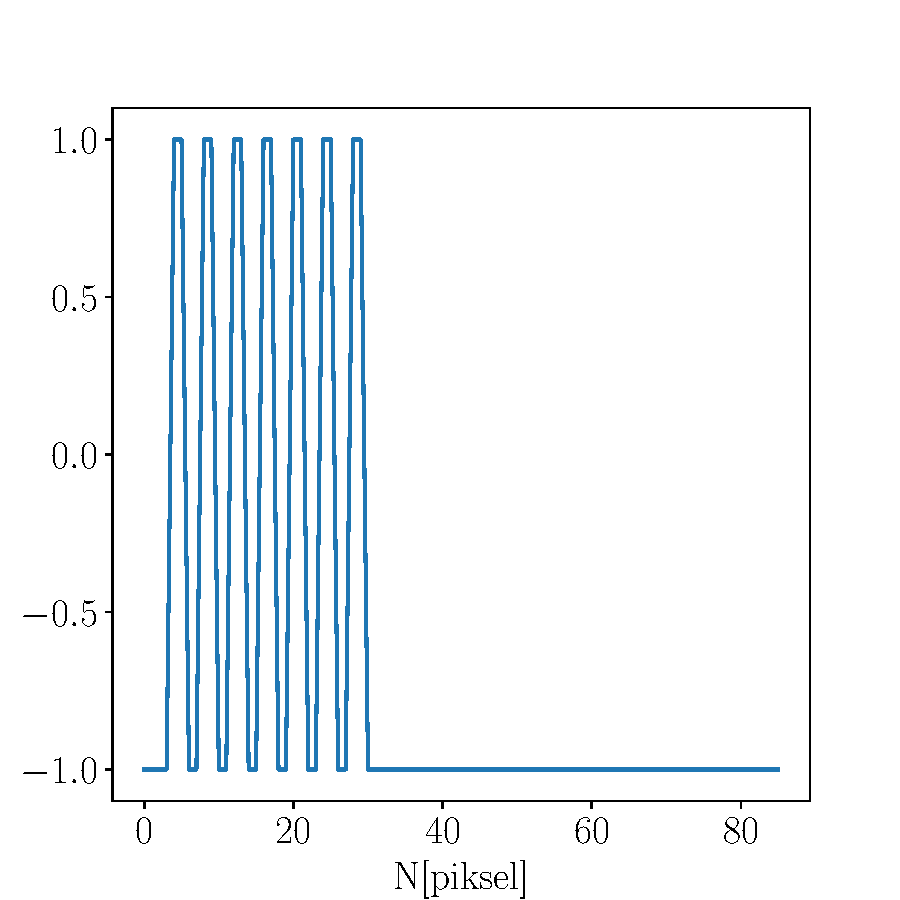
\includegraphics[width=\textwidth]{sync_frame0.pdf}
        \caption{Sinhronizacija A}
    \end{subfigure}
    \hfill
    \begin{subfigure}[b]{0.45\textwidth}
        \centering
        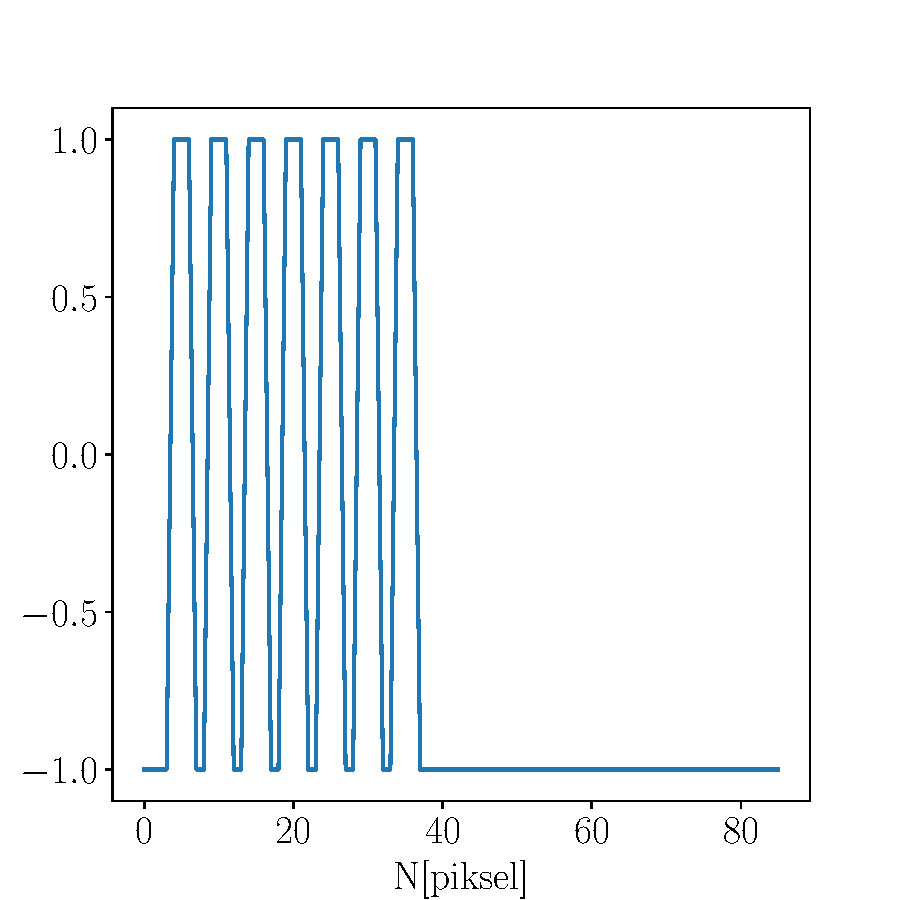
\includegraphics[width=\textwidth]{sync_frame1.pdf}
        \caption{Sinhronizacija B}
    \end{subfigure}

    \caption{Sinhronizaciji A in B s presledkom v obliki signala.}
    \label{fig:sync_frames}
\end{figure}
Za slikovni del si najprej izberemo sliki in ju spremenimo v format `grayscale` s širino $909$, kjer je vsak piksel predstavljen z vrednostjo med $0$ in $255$. Vrednosti nato normaliziramo na interval $-1$ in $1$. Tako s sinhronizacijskim delom in telemetrijo sestavimo signal za vsako vrstico, ki jih nato zaporedno združimo v sporočilni signal.

Za lažje oddajanje in sprejemanje je potrebna še amplitudna modulacija podatkov. Sestavljen signal, ki smo ga pridobili s prejšnjim postopkom označimo z $m(t)$ in predstavlja naše sporočilo. Za amplitudno modulacijo definiramo najprej nosilni val
\begin{equation*}
	c(t) = A \sin{(2\pi f_c t)}\text{,}
\end{equation*}
kjer je $f_c$ nosilna frekvenca in je v NOAA APT formatu enaka vrednosti $f_c=\SI{2400}{\hertz}$. S tem definiramo amplitudno modulacijo 
\begin{equation*}
	y(t) = (1 + km(t))c(t)\text{,}
\end{equation*}
kjer k definiramo kot modulacijski indeks z vrednostjo $k=0.7$ \cite{am_wiki}. Formulo nato diskretno uporabimo na celotnem signalu. Primer signala je na sliki \ref{fig:signal_example}. 
\begin{figure}[H]
    \centering
    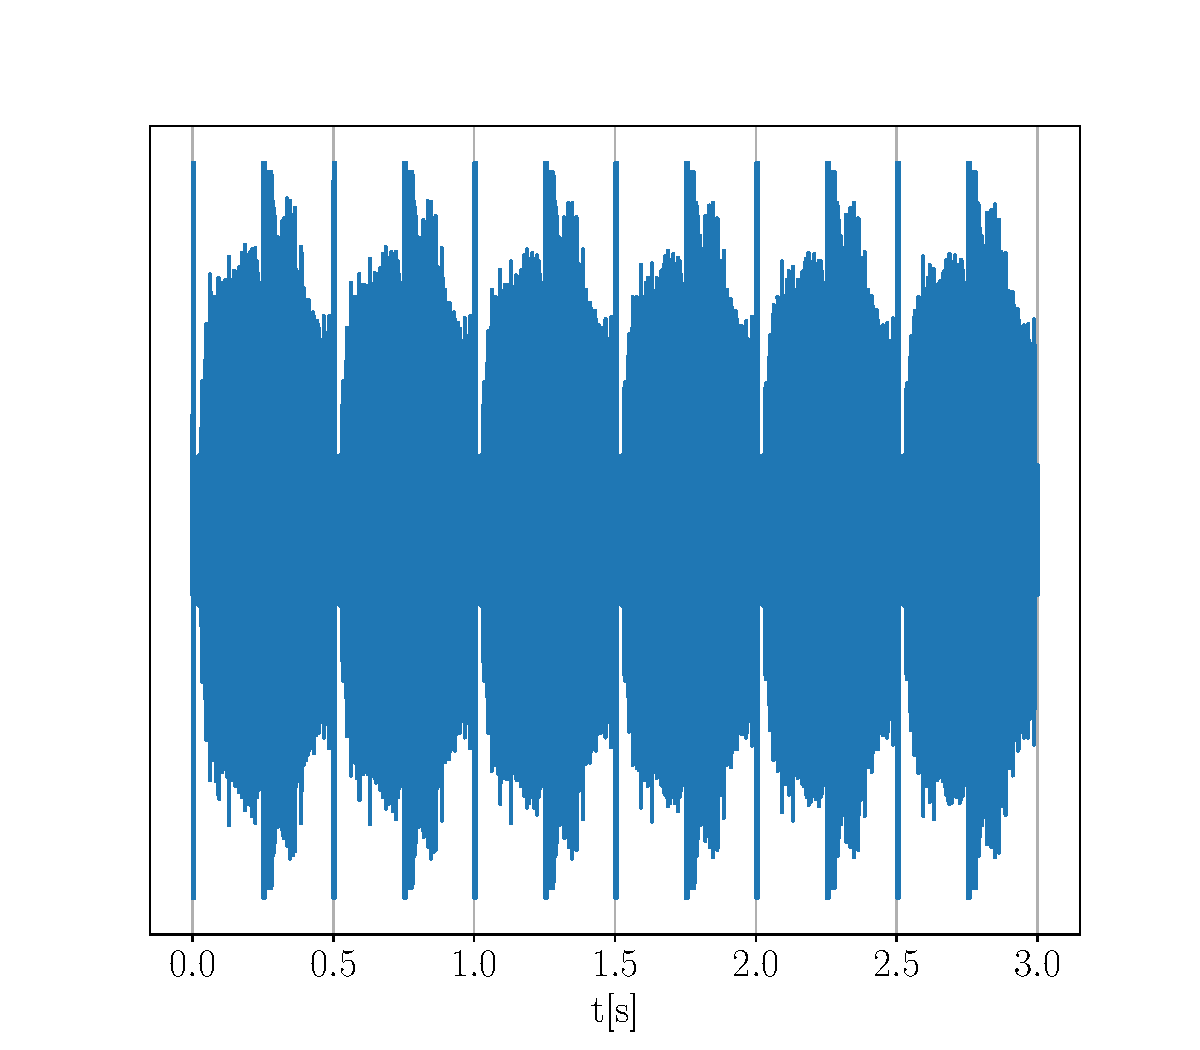
\includegraphics[width=0.5\textwidth]{signal_example.pdf}
    \caption{$\SI{3}{\second}$ izrez primera NOAA APT signala.}
    \label{fig:signal_example}
\end{figure}
Po tem postopku dobimo signal s frekvenco $\SI{4160}{\hertz}$, kar je precej majhna frekvenca, saj je že ustrezna Nyquistova frekvenca enaka $\SI{2180}{\hertz}$, kar je manjše od nosilne frekvence. Da povečamo frekvenco, lahko na začetku ustrezno spremenimo širino slike. V vzorcih za sinhronizacijo pa ponovimo posamezne piksle in tako ohranimo vzorec. 
\section{Dekodiranje}
Preden začnemo z dekodiranjem je smiselno preveriti ali posnetek sploh vsebuje željene podatke. To lahko storimo tako, da posnetek transformiramo v frekvenčno domeno s pomočjo hitre Fourierove transformacije in preverimo, da je vrh pri nosilni frekvenci. Na sliki \ref{fig:fft} lahko razberemo, da vrh spektra ustreza že prej omenjeni nosilni frekvenci $f_c=\SI{2400}{\hertz}$.
\begin{figure}[H]
    \centering
    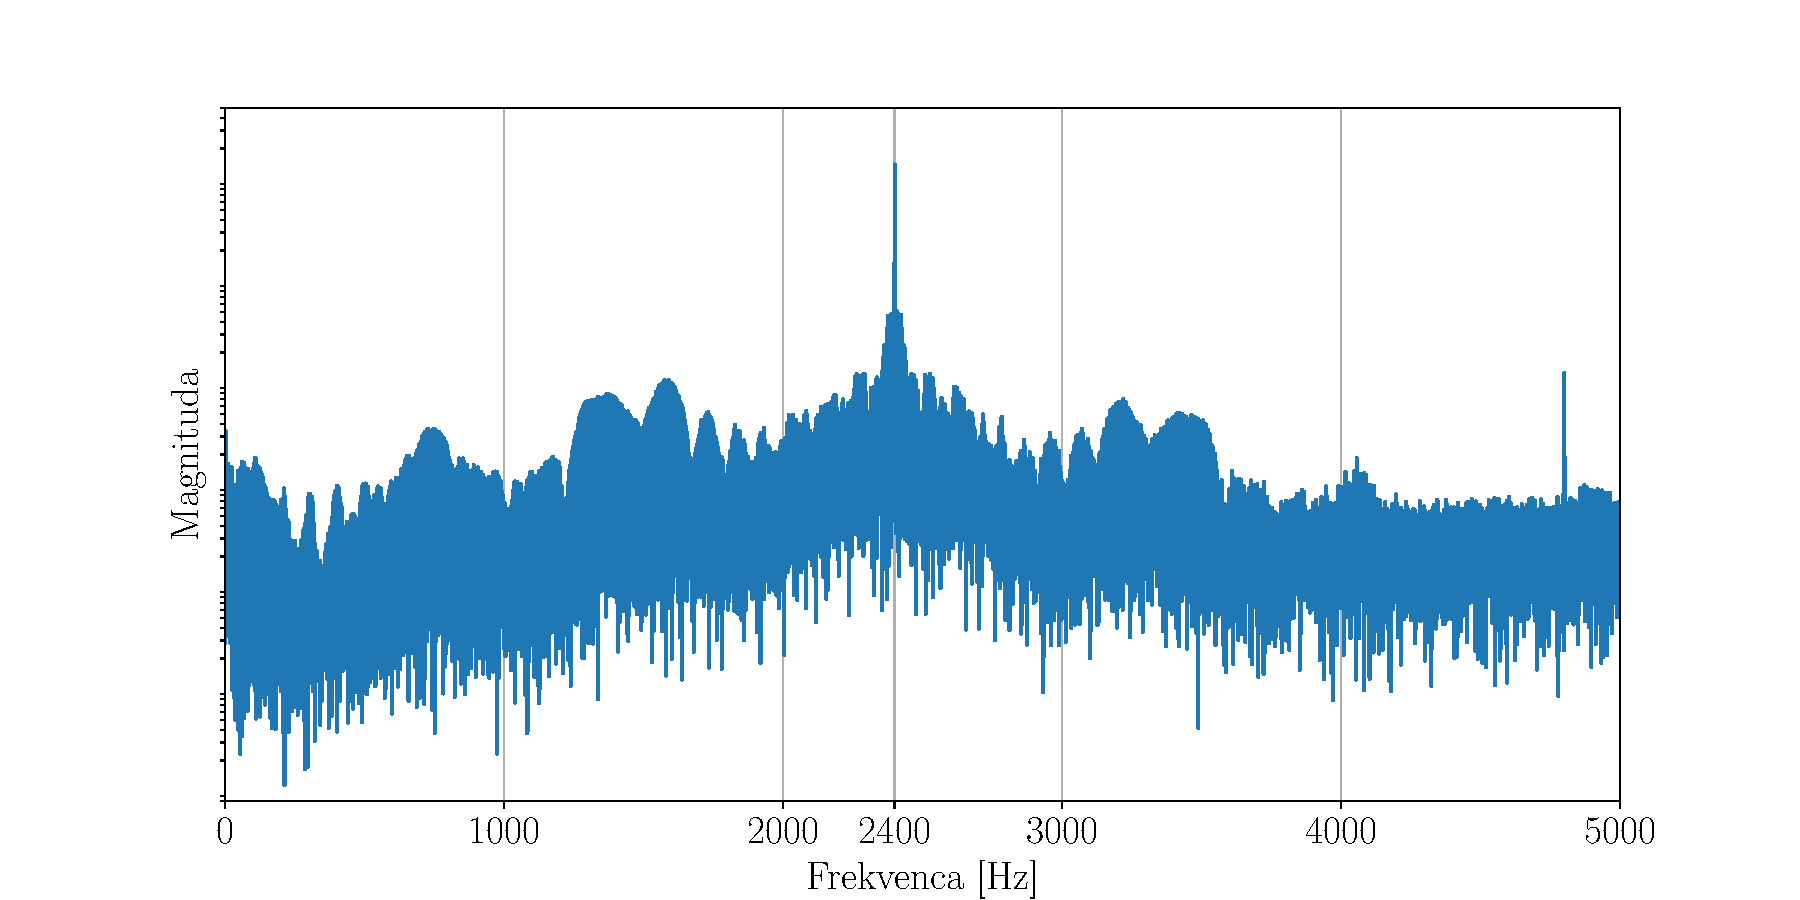
\includegraphics[width=1\textwidth]{fft_plot.pdf}
    \caption{Spekter vhodnega signala.}
    \label{fig:fft}
\end{figure}
Prvi korak dekodiranja je vzorčenje vhodnega posnetka iz vhodne frekvence $f_v$ na $f_i=\SI{20800}{\hertz}$. Da ne izgubimo informacije o sliki tega ne smemo storiti z vgrajeno funkcijo \texttt{resample}, saj ta uporablja Fourierovo transformacijo, ki predpostavi periodičnost signala. Temu se izognemo tako, da sledimo naslednjemu postopku:
\begin{itemize}
  \item Izračunamo interpolacijski faktor $L$ in decimacijski faktor $M$, ki čim bolje ustrezata okrajšanemu ulomku $f_i/f_v\approx L/M$.
  \item Sestaviš nizkopasovni filter s Kaiserjevim oknom in funkcijo sinc.
  \item Med vzorce vstavimo $L-1$ ničel in izvedemo konvolucijo z nizkopasovnim filtrom.
  \item Vzamemo vsak $M$-ti vzorec.
\end{itemize}
Naslednji korak je amplitudna demodulacija, h kateri pristopimo z vrednostima dveh zaporednih vzorcev
\begin{align*}
	y[i-1] = m[i-1]\sin{(2\pi f_c t_0 + \alpha)}\text{,} \\
	y[i] = m[i]\sin{(2\pi f_c (t_0 + \Delta t) + \alpha)}\text{.}
\end{align*}
Za nadaljevaje predpostavimo, da je $\Delta t$ majhen oziroma s predpostavko, da je vzorčna frekvenca visoka. S tem lahko rečemo, da je $m[i] \approx m[i-1]$ in izpeljemo naslednjo enačbo 
\begin{equation*}
	m[i] = \frac{\sqrt{y[i]^2 + y[i-1]^2-2y[i]y[i-1]\cos{\phi}}}{\sin{\phi}}\text{,}
\end{equation*}
kjer $\phi = 2\pi f_c/f_i$ \cite{bernardi}. Po končani amplitudni demodulaciji z že prej opisanim postopkom vzorčimo signal na $\SI{4160}{\hertz}$, kar je enako številu pikslov v eni sekundi.
Preostane še iskanje sinhronizacije v signalu, da najdemo začetek vsake vrstice. To storimo s pomočjo križne korelacije
\begin{equation*}
	(f \star g)[n] = \sum_{m=0}^{N-1} \overline{f[m]} \, g\bigl[(m+n)_{\text{mod}\, N}\bigr],
\end{equation*}
 ki je mera podobnosti. V našem primeru namesto funkcije $g[i]$ uporabimo sinhronizacijo A na sliki \ref{fig:sync_frames} in za $f[i]$ amplitudno demoduliran signal $m[i]$.
\begin{figure}[H]
    \centering
    \begin{subfigure}[b]{0.49\textwidth}
        \centering
        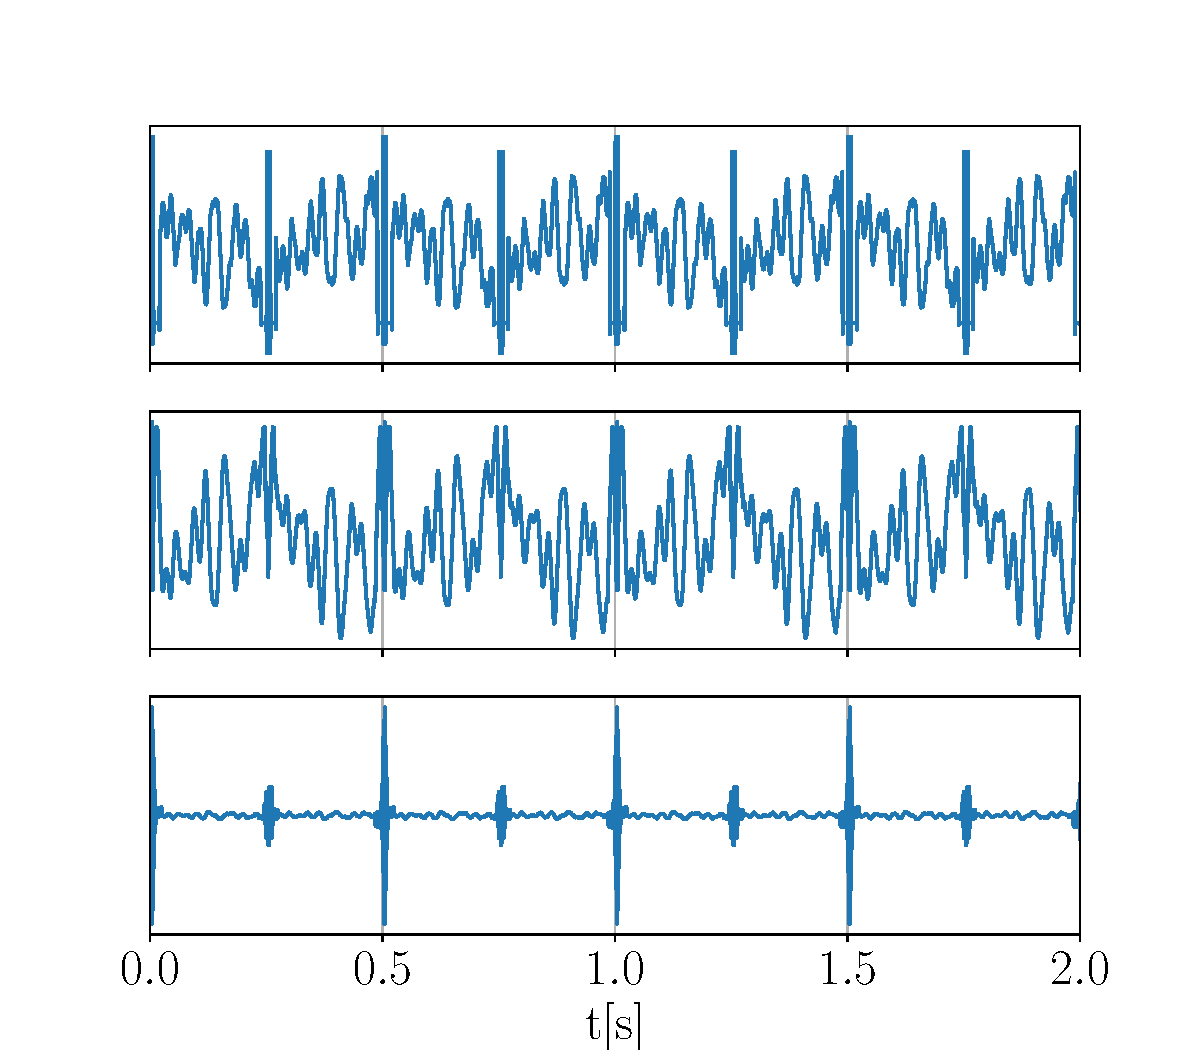
\includegraphics[width=\textwidth]{penguin_corr.pdf}
        \caption{Generiran signal.}
    \end{subfigure}
    \hfill
    \begin{subfigure}[b]{0.49\textwidth}
        \centering
        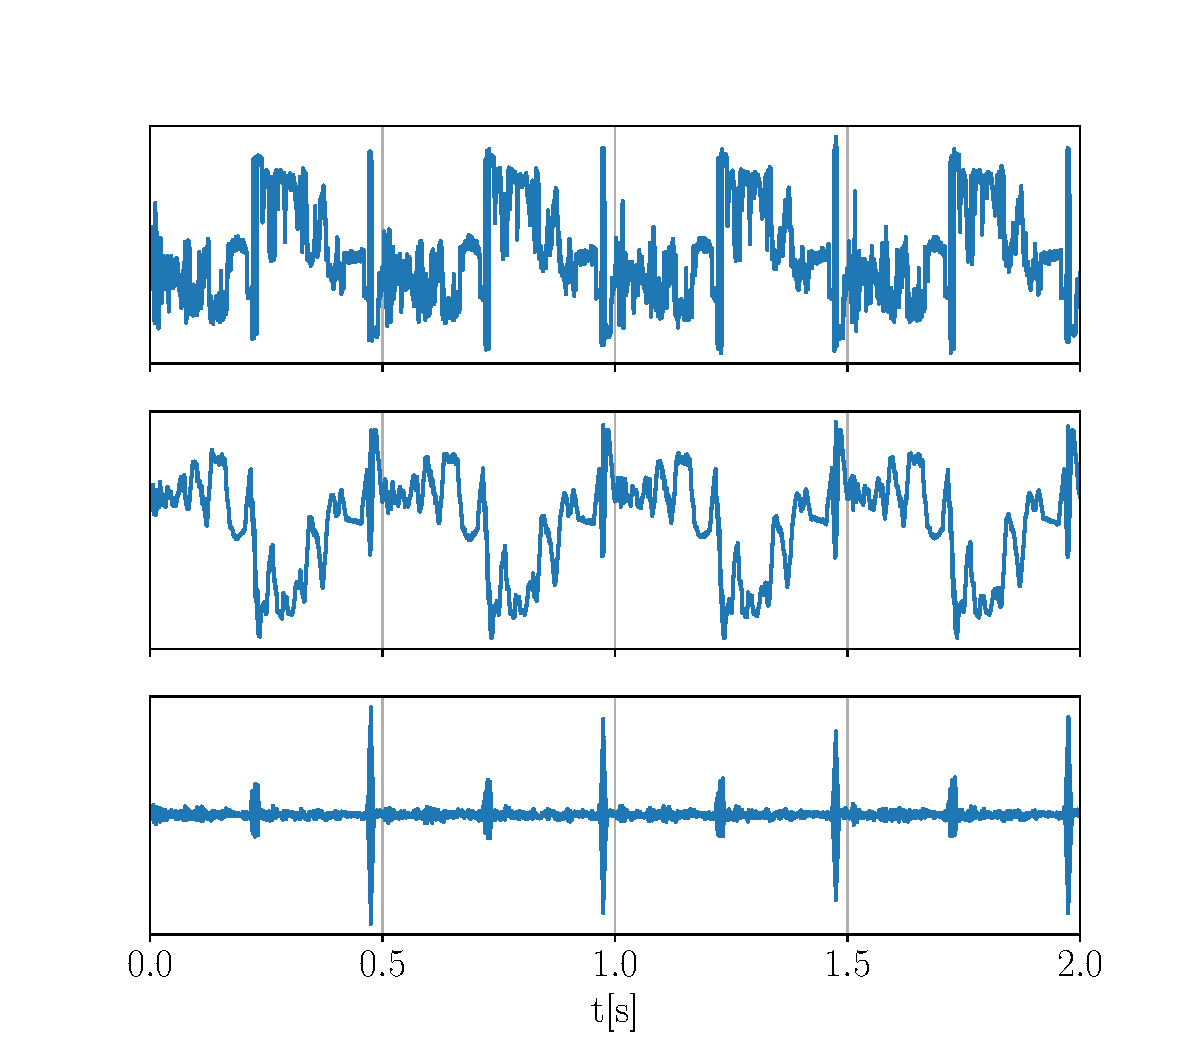
\includegraphics[width=\textwidth]{argentina_corr.pdf}
        \caption{Posneti signal.}
    \end{subfigure}

	\caption{V zgornji sliki je demoduliran signal, v srednji signal koreliran s sinhronizacijo A, in v spodnji razlika med sosednjima vzorcema koreliranega signala s sinhronizacijo A.}
    \label{fig:sync_corr}
\end{figure}
V koreliranem rezultatu opazimo, da pričakovano, vrednost okoli točke, kjer se nahaja sinhronizacija narašča. V prvi iteraciji smo uporabili kot začetek vrstice maksimum korelacije v intervalu $2080$ pikslov. To je imelo kar precej težav, saj kot vidimo v generiranem signalu ima precej visoko vrednost tudi korelacija ob sinhronizaciji B. V izogib temu pogledamo razliko med sosednjima vrednostima. S tem dobimo v intervalu $2080$ pikslov dva vrhova. Prvi, ki je na sliki \ref{fig:sync_corr} jasno večji pripada sinhronizaciji A in drugi manjši pripada sinhronizaciji B. Tako lahko iz slike \ref{fig:sync_corr} razberemo, da se pri generiranem signalu kot pričakovano vrhovi ujemajo z intervalom $\SI{0.5}{\second}$. Na posnetem signalu pa opazimo, da je signal rahlo zamaknjen in se vsaka vrstica začne malo pred začetkom intervala $\SI{0.5}{\second}$ glede na čas v posnetku.

Vsako vrstico nato pretvorimo v sliko tako, da normaliziramo glede na najmanjšo in največjo vrednostjo in porazdelimo vrednosti amplitude med $0$ in $255$ ter tako spremenimo signal v `grayscale` format slike. Običajno bi tu za translacijo amplitude v `grayscale` uporabili vrednosti iz telemetrije, ki bi določila točne vrednosti, a je za potrebe te naloge normalizacija delovala dovolj dobro.
\newpage
\section{Rezultati}
Poglejmo še nekaj slik, ki jih na tak način dekodiramo iz posnetih signalov. 
\begin{figure}[H]
    \centering
    \begin{subfigure}[b]{0.49\textwidth}
        \centering
        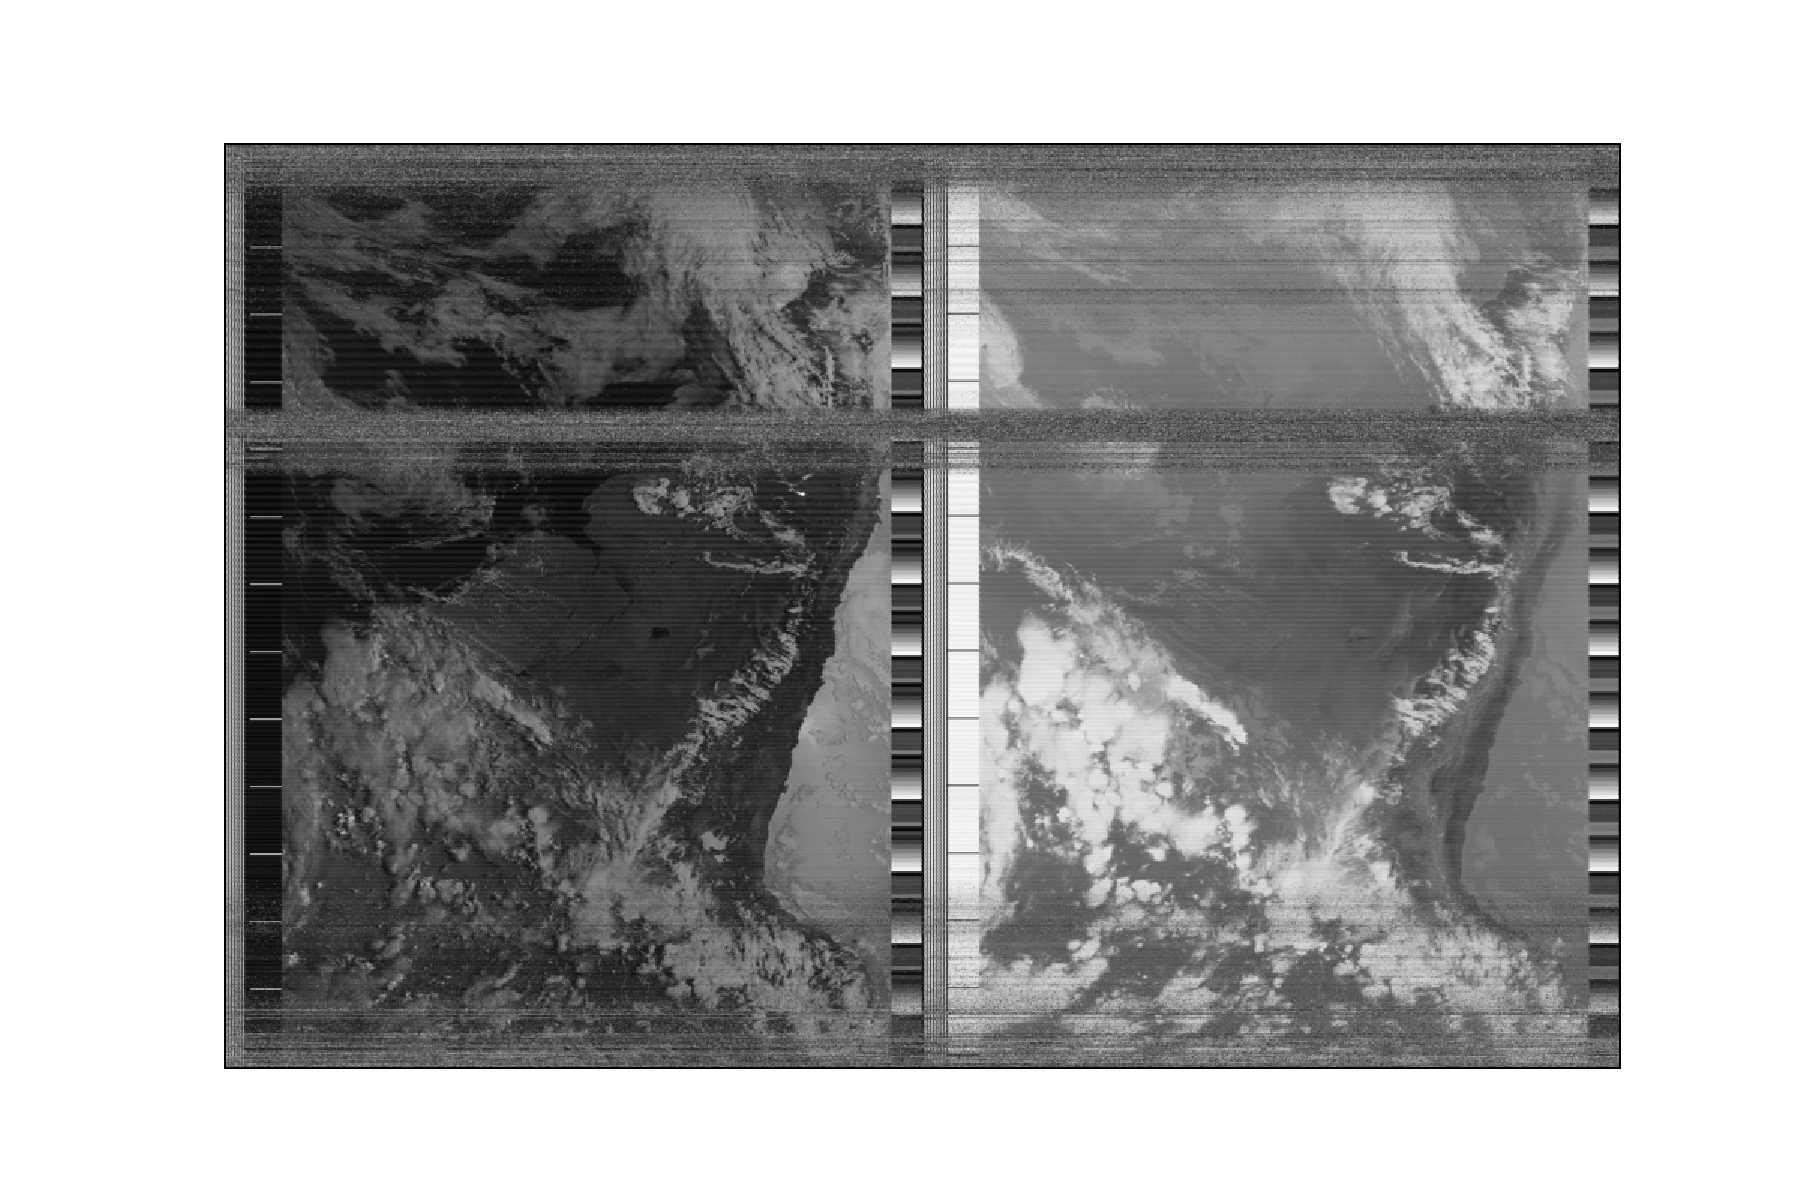
\includegraphics[width=\textwidth]{argentina.pdf}
        \caption{Argentina}
    \end{subfigure}
    \hfill
    \begin{subfigure}[b]{0.49\textwidth}
        \centering
        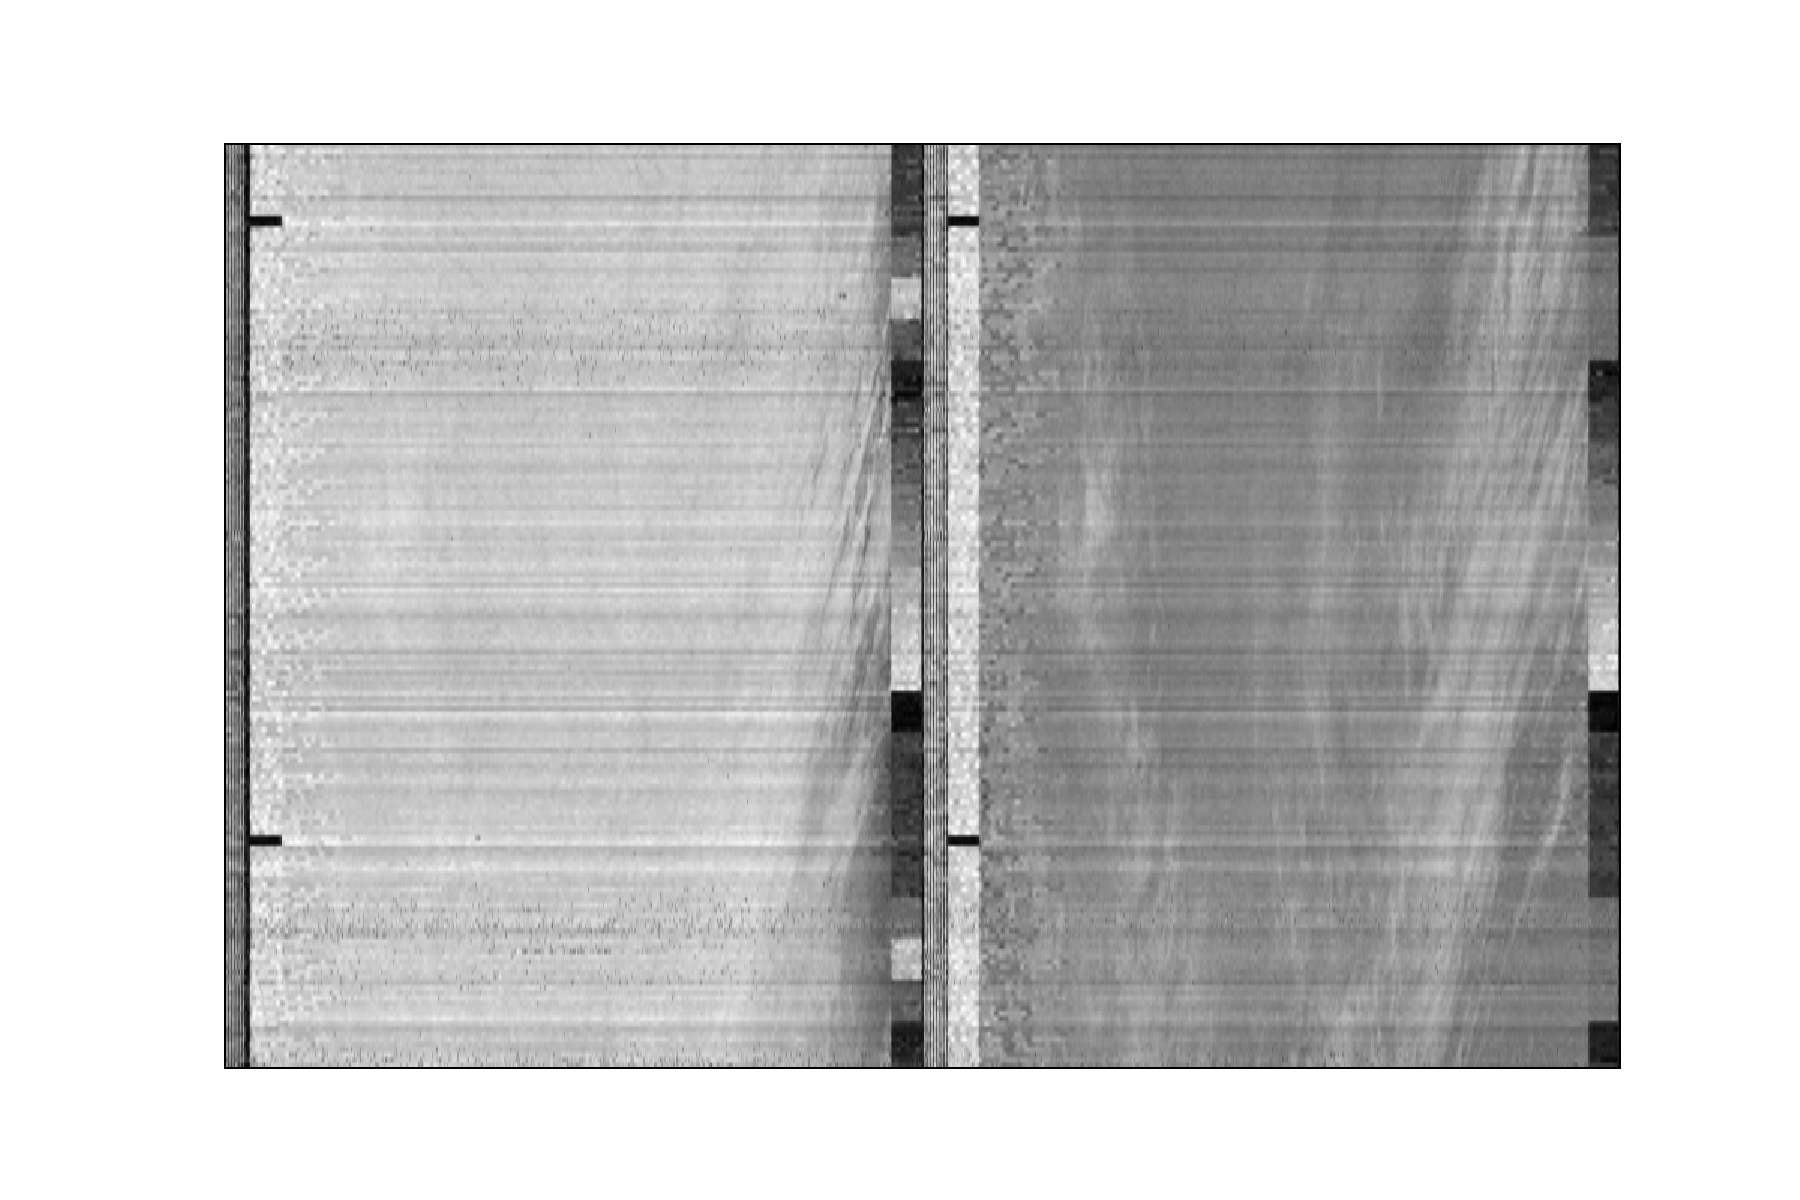
\includegraphics[width=\textwidth]{belgium.pdf}
        \caption{Belgija}
    \end{subfigure}

	\caption{Signala posneta iz NOAA satelitov nad Argentino in Belgijo.}
    \label{fig:out_example}
\end{figure}
Še en primer posnet nad Slovenijo.
\begin{figure}[H]
    \centering
    \begin{subfigure}[b]{0.8\textwidth}
        \centering
        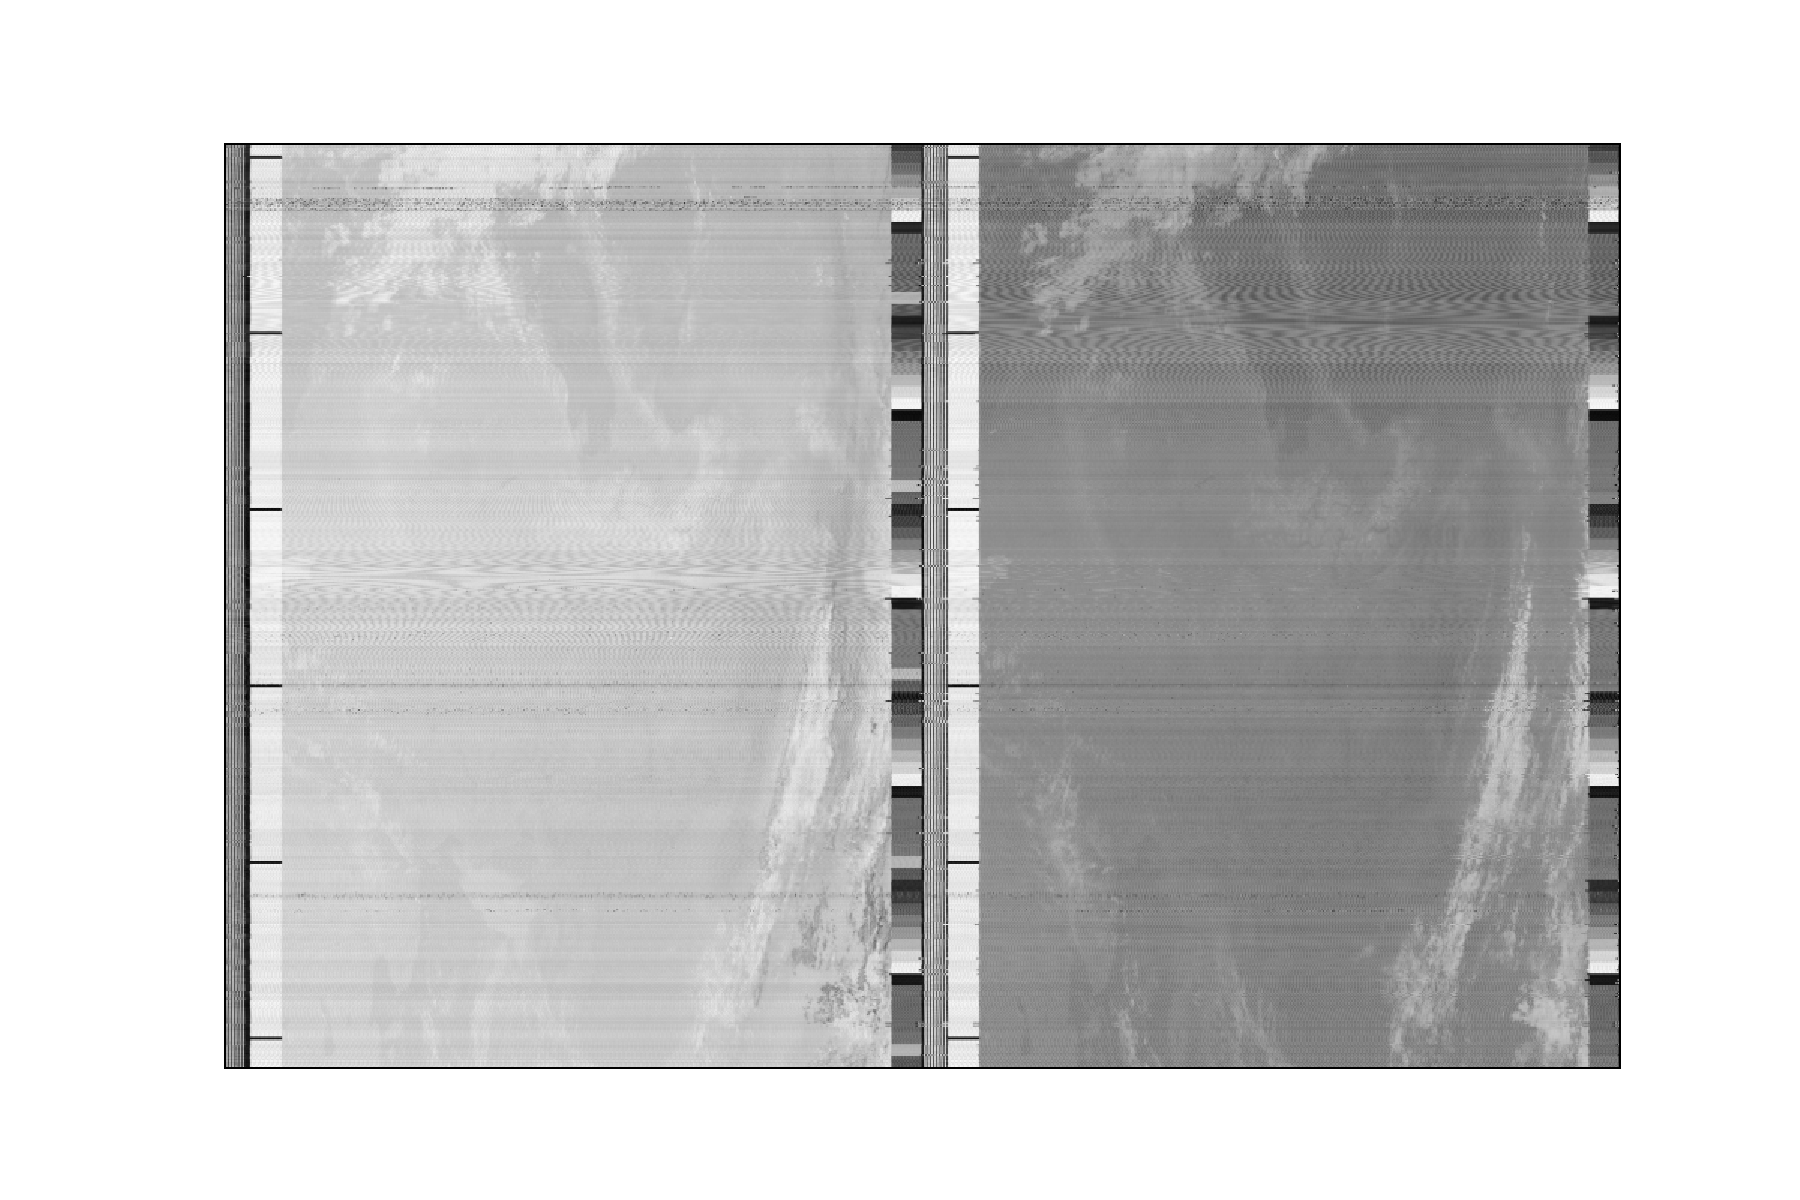
\includegraphics[width=\textwidth]{slovenia.pdf}
        \caption{Argentina}
    \end{subfigure}
	\caption{Signal posnet iz NOAA satelita nad Slovenijo.}
    \label{fig:out_example}
\end{figure}
\newpage
Za konec pa še nekaj enkodiranih in nato dekodiranih slik, kjer je slika v kanalu B inverz slike v kanalu A. 
\begin{figure}[H]
    \centering
    \begin{subfigure}[b]{0.49\textwidth}
        \centering
        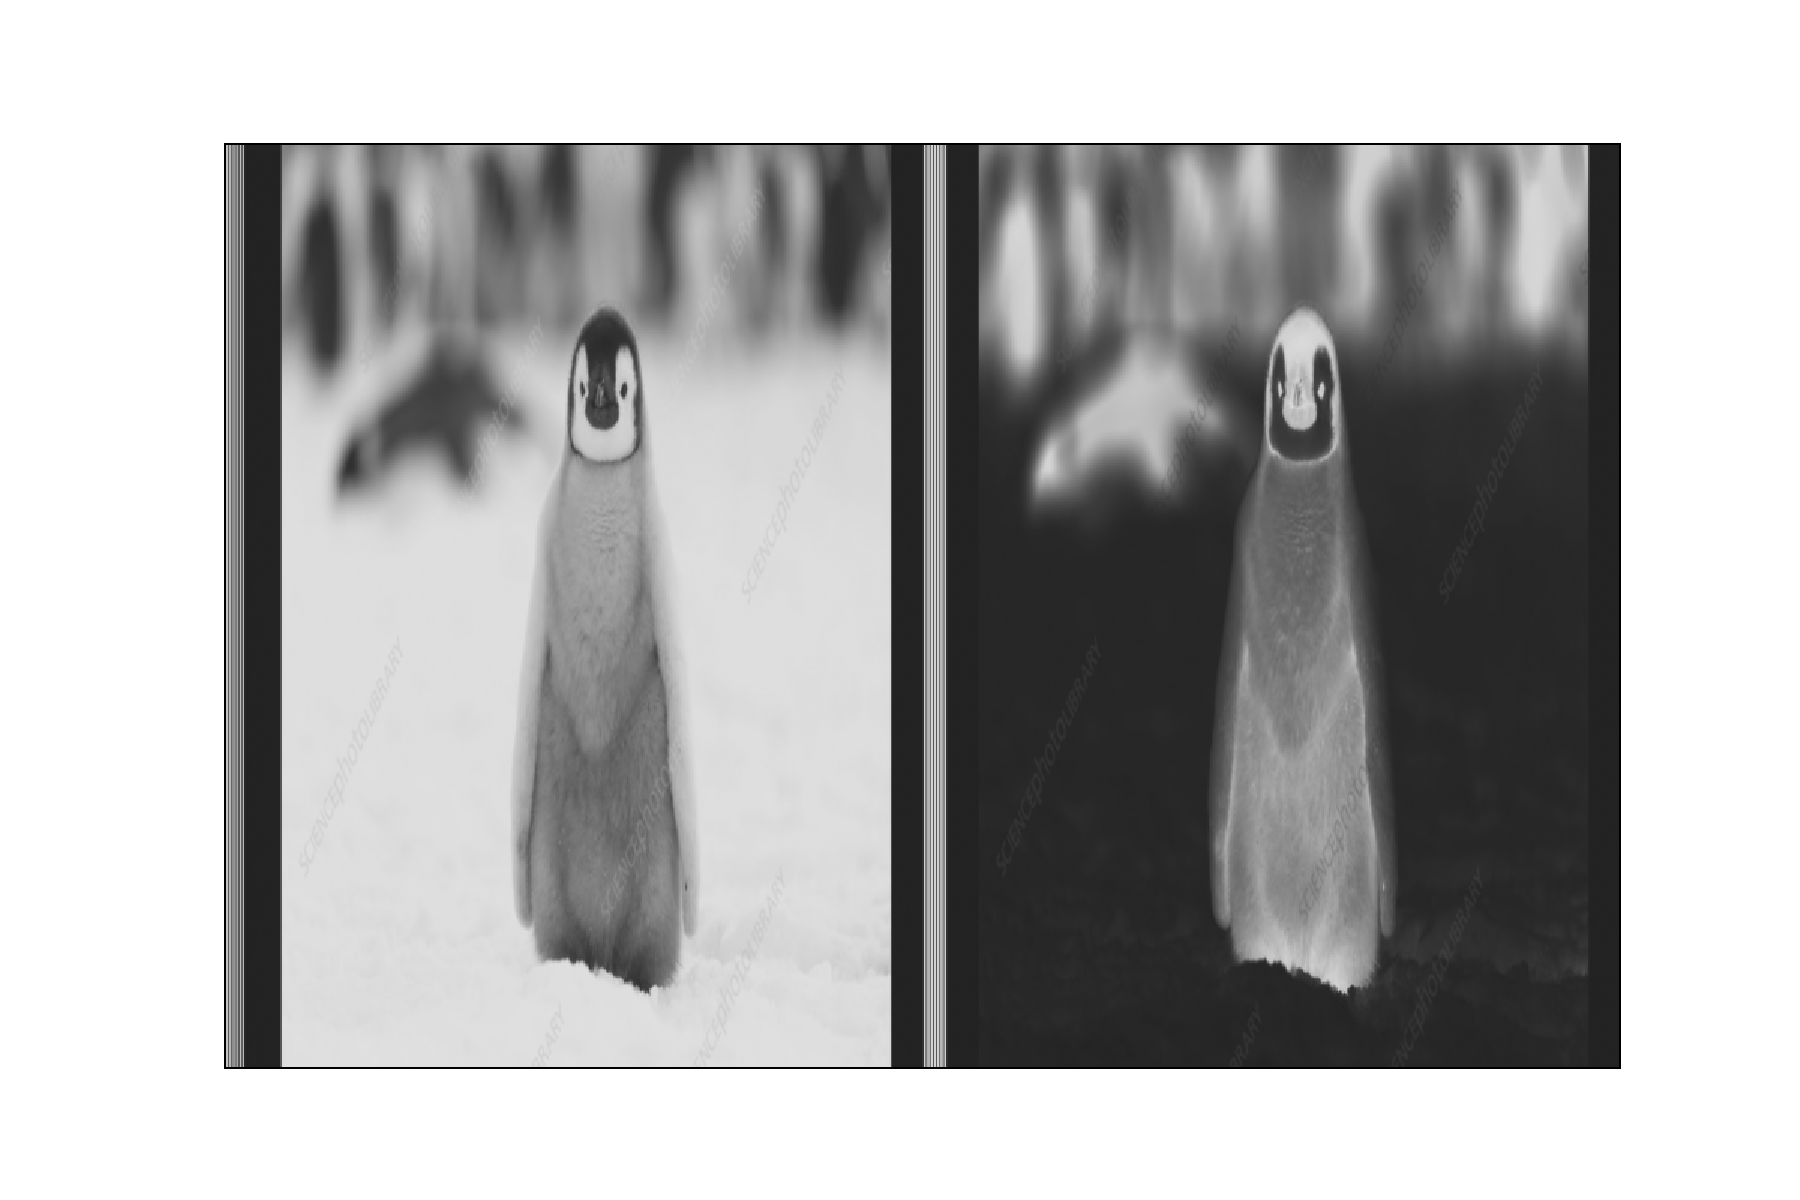
\includegraphics[width=\textwidth]{penguin.pdf}
    \end{subfigure}
    \hfill
    \begin{subfigure}[b]{0.49\textwidth}
        \centering
        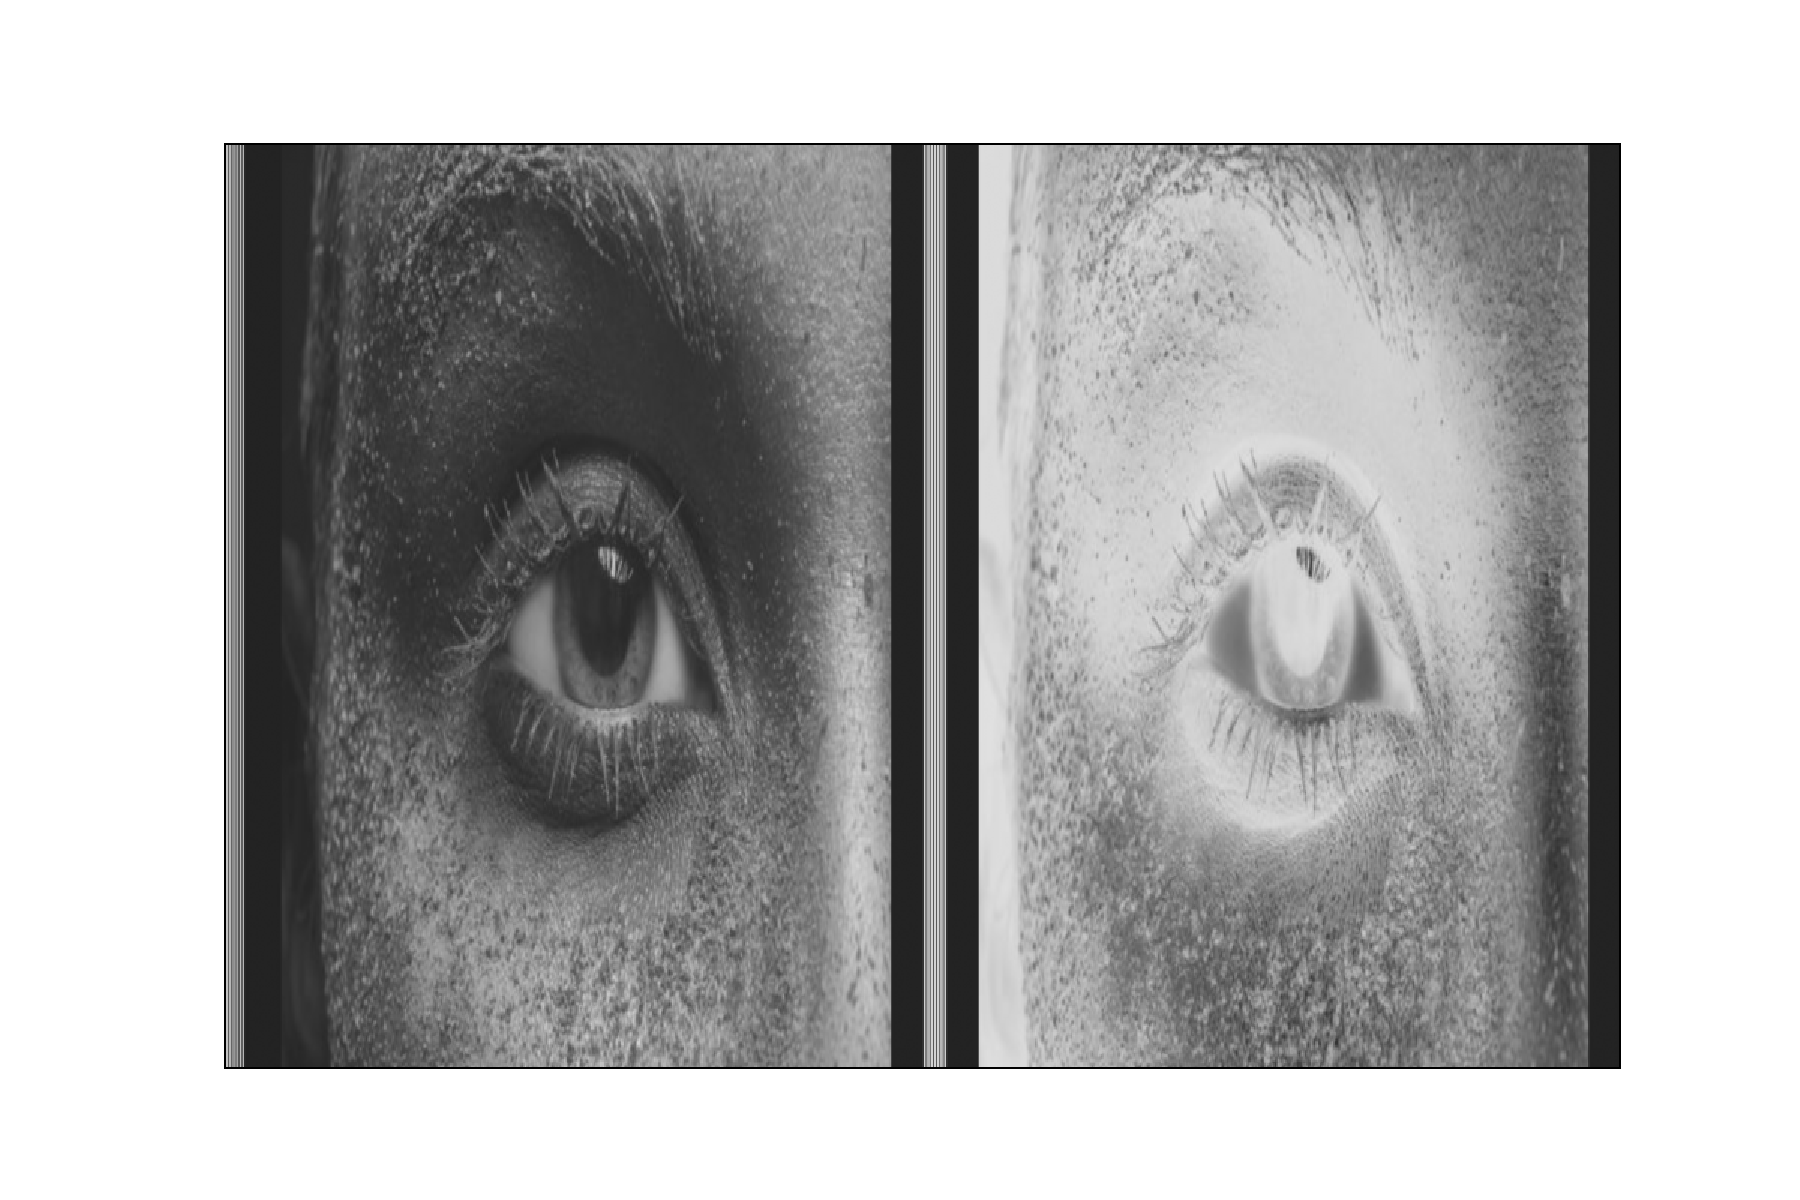
\includegraphics[width=\textwidth]{eye.pdf}
    \end{subfigure}
	\caption{Dekodirana generirana signala iz poljubne slike, kjer je v kanalu A originalna slika v kanalu B pa njen inverz.}
    \label{fig:out_example}
\end{figure}
\section{Zaključek}
V tem poročilu smo obravnavali koncepte potrebne za kodiranje in dekodiranje signala NOAA APT in si na koncu ogledali nekaj primerov slik, ki jih dobimo preko tega postopka. V nadaljevanju bi lahko implementirali še telemetrijski del podatkov in frekvenčno modulacijo oziroma demodulacijo. Lahko bi tudi poskusili razširiti format tako, da bi v vsakega izmed kanalov shranili podatek o eni barvi in ju nato v dekodiranju združili v eno sliko.


\printbibliography[heading=bibnumbered]
\end{document}

